\chapter{Lezione 4 - Memorie ad accesso casuale}

In questa lezione ci occupiamo delle memorie ad accesso casuale, anche chiamate RAM.

\FloatBarrier
\begin{figure}[H]
  \centering
  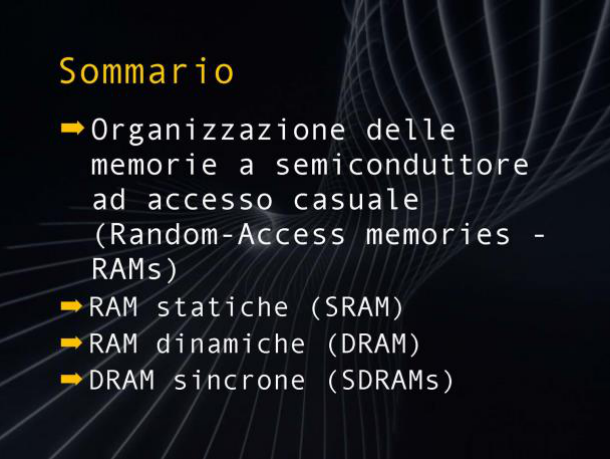
\includegraphics[width=0.40\textwidth,
                    trim=40 40 10 40, % L B R T
                    clip]
                    {images/Lez04_p01_fig_02.png}
  \caption{Sommario}
  \label{fig:Lez04_p01_fig_02}
\end{figure}
\FloatBarrier
\noindent

Ci occuperemo dell'organizzazione delle memorie a semiconduttore ad accesso casuale, chiamate anche Random Access Memories o RAMs in inglese.
Ci occuperemo delle RAM statiche, chiamate anche SRAM, delle RAM dinamiche o RAM, delle RAMs sincrone o chiamate anche SRAM.

Cominciamo con l'organizzazione delle memorie ad accesso casuale in termini generali.

\FloatBarrier
\begin{figure}[H]
  \centering
  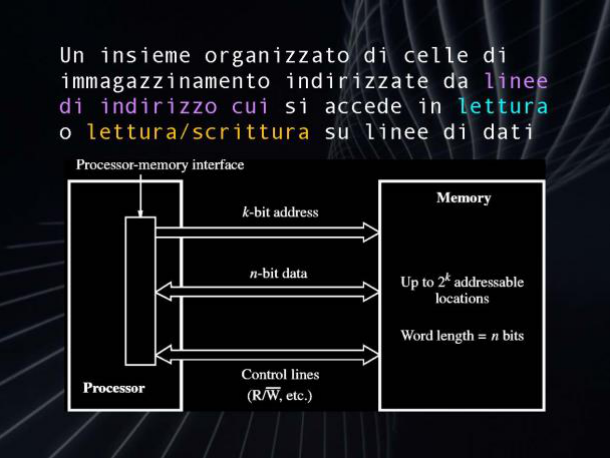
\includegraphics[width=0.60\textwidth,
                    trim=40 20 10 40, % L B R T
                    clip]
                    {images/Lez04_p01_fig_04.png}
  \caption{Sommario}
  \label{fig:Lez04_p01_fig_04}
\end{figure}
\FloatBarrier
\noindent

Questo è un insieme di celle di immagazzinamento indirizzate da linee di indirizzo a cui si accede in lettura oppure in lettura e scrittura su linee di dati.
Questo è il concetto generale di una memoria indirizzata mediante righe e colonne.
Ci sono delle righe dei segnali di indirizzo che identificano locazioni all'interno di questa memoria.
In generale vi sarà un processore che produce una richiesta.
Questa richiesta è gestita da un'interfaccia memoria-processore.

Da questa interfaccia partono k-line di indirizzo, quindi k-fili sostanzialmente, che identificano k-bit di indirizzo.
c'è un canale generalmente bidirezionale, dove sia prevista la lettura e scrittura, in cui transitano i dati.
Vi sono in fine un insieme di linee di controllo, per esempio le linee che danno il comando se si tratti di lettura read o scrittura write.
È comune questa terminologia read-write complementato per indicare che con il segnale alto è un read e con il segnale basso è un write, cioè una scrittura.
La memoria è in questo momento una scatola costituita da due alla k-locazioni indirizzabili dai questi k-bit di indirizzo.
La parola ha una lunghezza di n-bit e potrà transitare in una direzione e o nell'altra attraverso gli n-bit di i-dato.

\FloatBarrier
\begin{figure}[H]
  \centering
  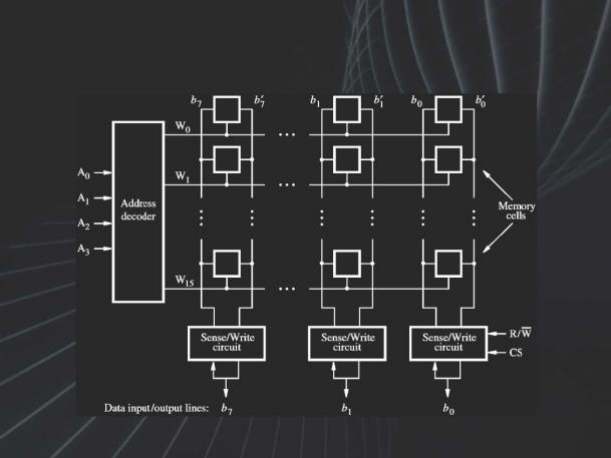
\includegraphics[width=0.80\textwidth,
                    trim=40 40 10 40, % L B R T
                    clip]
                    {images/Lez04_p01_fig_05.png}
  \caption{Semplice memoria}
  \label{fig:Lez04_p01_fig_05}
\end{figure}
\FloatBarrier
\noindent

Vediamo adesso una semplice memoria, ma che è esemplificativa, in cui abbiamo 8-bit di dato da b0 a b7, acceduti da due linee b0 negato, b1 negato, b7 negato e indirizzata da dei segnali w0 w15 che sono decodificati da un decoder a 4 ingressi e 16 uscite $2^4$.

Ognuno delle celle di locazione b0 indirizzata da w0, b0 indirizzato da w1, giù fino a b0 indirizzata da w15, ha un comune circuito di sense write, cioè di lettura e scrittura, sostanzialmente un insieme di stati di scrittura, cioè di amplificatori in scrittura e amplificatori comandati da appositi segnali read write negato e appositi segnali chip select.

All'ingresso e all'uscita di questo stadio di sense write è posto il bit 0 che proviene dalle linee di dato nel caso si tratti di una scrittura o che arriverà sulle linee di dato nel caso si tratti di una lettura notate e la freccia bidirezionale.

I segnali di read write e chip select sono applicati ugualmente a tutti i circuiti di sense write.

In questo semplice caso abbiamo 8 bit indirizzati contemporaneamente da un segnale decodificato dal decoder indirizzi. Questa è una semplice memoria 16 per 8 bit.

\FloatBarrier
\begin{figure}[H]
  \centering
  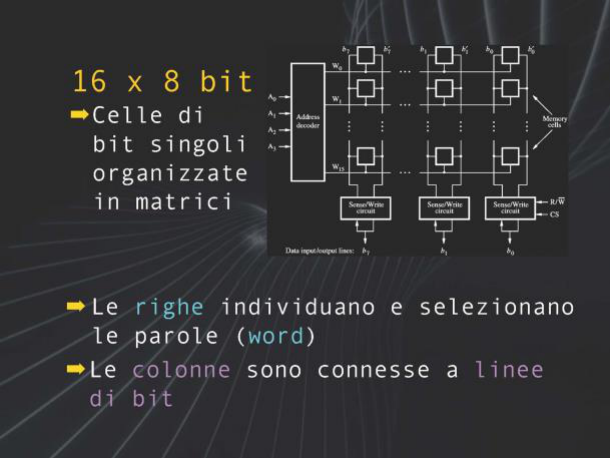
\includegraphics[width=0.60\textwidth,
                    trim=40 40 10 40, % L B R T
                    clip]
                    {images/Lez04_p01_fig_06.png}
  \caption{Memoria 16x8bit}
  \label{fig:Lez04_p01_fig_06}
\end{figure}
\FloatBarrier
\noindent

Ovviamente in questa figura abbiamo rappresentato una memoria che sia graficamente rappresentabile sullo schermo ma ovviamente potete estendere questo concetto a numeri ben più grandi come avviene nelle comuni applicazioni oggigiorno.
Le celle di bit singole sono quindi organizzate topologicamente in matrici.
Le righe individuano e selezionano le parole o word in inglese.
Le colonne sono connesse a linee di bit.
Questo è l'approccio a livello matriciale in cui tutto l'indirizzo è spezzato solo lungo una dimensione per definire ed abilitare questi elementi di memoria che al momento sono ancora delle scatole oscure.

\FloatBarrier
\begin{figure}[H]
  \centering
  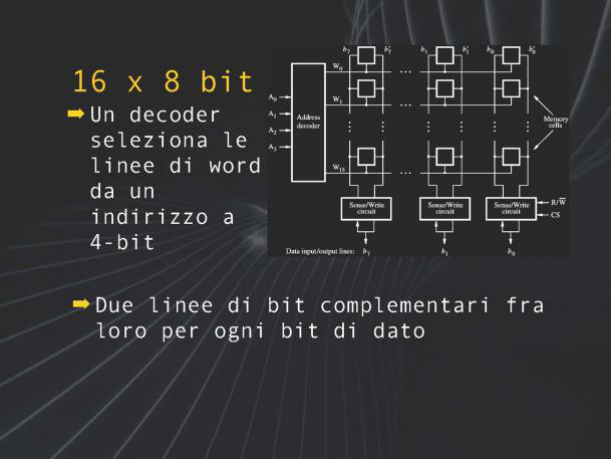
\includegraphics[width=0.60\textwidth,
                    trim=40 40 10 40, % L B R T
                    clip]
                    {images/Lez04_p02_fig_01.png}
  \caption{Memoria 16x8bit}
  \label{fig:Lez04_p02_fig_01}
\end{figure}
\FloatBarrier
\noindent

È importante osservare che il decoder che decodifica gli indirizzi che sono codificati binariamente in queste 4 linee.
2 alla 4 fa 16 quindi si va da 0 a 16 linee decodificate che selezionano gli elementi di memoria sulle 16 diverse parole.
In questo caso usiamo due linee di bit complementari fra loro per ogni bit di dato. Leveremo questo vincolo fra poco.

\FloatBarrier
\begin{figure}[H]
  \centering
  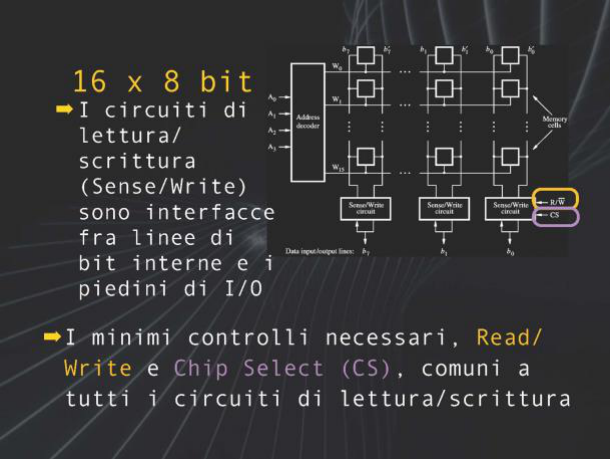
\includegraphics[width=0.60\textwidth,
                    trim=40 40 10 40, % L B R T
                    clip]
                    {images/Lez04_p02_fig_02.png}
  \caption{Memoria 16x8bit}
  \label{fig:Lez04_p02_fig_02}
\end{figure}
\FloatBarrier
\noindent


I circuiti lettura e scrittura sono delle interfacce fra le linee di bit interne e i piedini di I/O, sostanzialmente sono degli amplificatori con degli elementi che possono essere controllati in una direzione o nell'altra.
Per far funzionare questo circuito i minimi controlli necessari sono read write e chip select che abilitano o disabilitano questi chip e sono comuni a tutti i circuiti lettura e scrittura come vi ho anticipato.

\FloatBarrier
\begin{figure}[H]
  \centering
  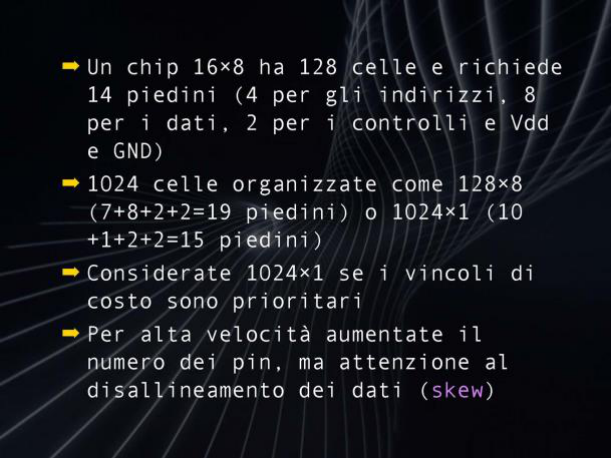
\includegraphics[width=0.60\textwidth,
                    trim=40 40 10 40, % L B R T
                    clip]
                    {images/Lez04_p02_fig_03.png}
  \caption{Memoria 16x8bit}
  \label{fig:Lez04_p02_fig_03}
\end{figure}
\FloatBarrier
\noindent

Un chip di 16x8 ha quindi 128 celle e richiede 14 piedini.
Il conteggio è semplice che ci sono 4 pin per gli indirizzi, 8 per i dati, 2 per i controlli read write e chip select e 1 per VDD e 1 per GND cioè la massa.

1024 celle possono quindi essere organizzate o come 128x8 oppure come 1024x1 con un numero di piedini in questo caso inferiore.
Il numero di piedini è pari a 10 perché 1024 è pari a $2^10$ più 1 pin di dato più 2 pin di controllo più alimentazione e massa fanno 15.
Vedete quindi che si possono fare delle scelte di progetto per definire il livello di parallelismo dei dati in uscita e questo ha un costo in termini di pin quando il parallelismo è più elevato e risparmia piedini in generale nei casi in cui non si abbiano questa esigenza.

Quindi considereremo un basso parallelismo se i vincoli di costo sui piedini sono dominanti oppure se vogliamo elevare la velocità aumenteremo il numero dei pin ma bisogna anche stare attenti al cosiddetto skew o disallineamento dei dati.
Notate infatti che questo è un problema particolarmente critico quando si aumenta la frequenza dei segnali che transitano sulle piste e le piste possono ad esempio avere diversi percorsi.

Immaginate una semplice curva che connette un piedino se avete tante piste in parallelo le piste che fanno come dire il giro corto all'interno della curva hanno un percorso inferiore alle piste che sono sul lato esterno della curva così come avviene in un normale ad esempio nella pista di atletica dove i corridori sulla pista interna se partono dalla stessa linea di partenza e arrivano alla stessa linea di partenza percorrerebbero un percorso più corto e quindi sarebbero avvantaggiati.

Questo va gestito opportunamente nei circuiti integrali dove si realizzano sistemi ad elevata velocità ne parleremo nella lezione successiva però richiamo la vostra attenzione sul fatto che aumentando il parallelismo si può aumentare la banda ma in generale bisogna aumentare maggiormente le precauzioni per evitare che i dati arrivino disallineati fra la sorgente e la destinazione.

\FloatBarrier
\begin{figure}[H]
  \centering
  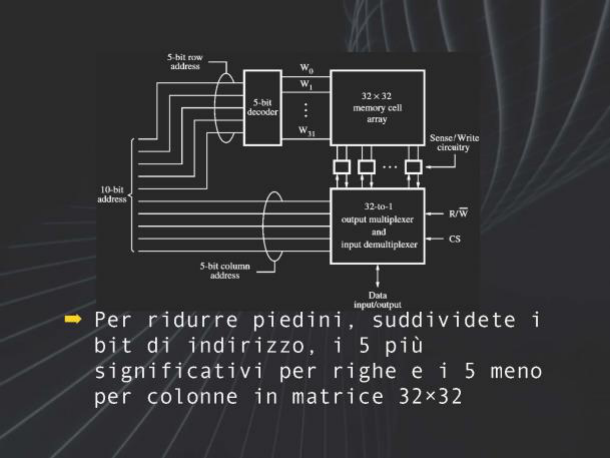
\includegraphics[width=0.80\textwidth,
                    trim=40 40 10 40, % L B R T
                    clip]
                    {images/Lez04_p02_fig_04.png}
  \caption{Riduzione numero pin}
  \label{fig:Lez04_p02_fig_04}
\end{figure}
\FloatBarrier
\noindent

Vediamo ora come si può ulteriormente ridurre il numero dei pin in un'architettura di una memoria.
Abbiamo visto che nel caso precedente semplice di un 16x8 avevamo 4 piste di indirizzo di dato.

Nel caso il numero delle piste di dato aumenti si possono partizionare le linee di dato, in questo caso vediamo 10 linee di dato, le possiamo partizionare in modo da averne 5 e 5 separate, quindi 5 andranno a costituire le cosiddette righe e 5 andranno a costituire le cosiddette colonne, non ci confondiamo con i segnali di dato, queste sono linee di indirizzo separate, quindi le più significative ad esempio sono quelle di righe e le meno significative quelle di colonna.

5 linee messe in un decoder producono 32 segnali, 5 linee messe in un multiplexer 32 in 1 decodificano questi circuiti di sense and write gli stessi che avevamo prima però ne abbiamo in questo caso 32.
Vengono multiplexati attraverso questo multiplexer 32 in 1 e 1 in 32, bilidirezionale, cioè di fatto sono due multiplexer capovolti messi l'uno contro l'altro e i dati transitano attraverso questa porta bilidirezionale ancora read write e chip select, questo cosa fa?
Permette di ridurre il numero delle piste di fatto sostanzialmente alla metà delle piste di indirizzo, quindi si suddividono i piedini di indirizzo, 5 più significativi per le righe e 5 meno significativi per le colonne e si organizza la parola in array di 32x32.
Un modulo di memoria di questo tipo può essere affiancato ad altri moduli di memoria per costruire gerarchie di memoria più elevata.

\FloatBarrier
\begin{figure}[H]
  \centering
  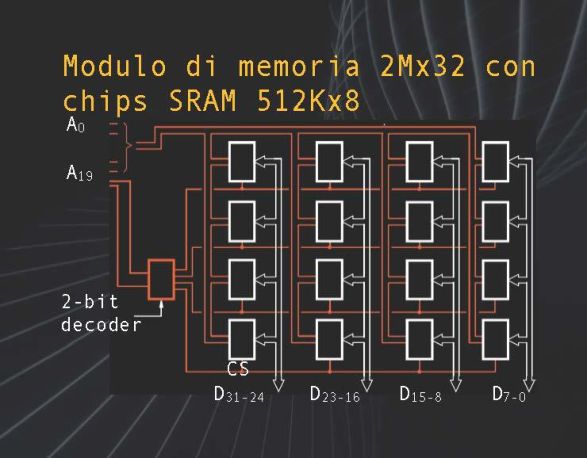
\includegraphics[width=0.80\textwidth,
                    trim=40 40 10 40, % L B R T
                    clip]
                    {images/Lez04_p02_fig_05.png}
  \caption{Memoria 2Mx32}
  \label{fig:Lez04_p02_fig_05}
\end{figure}
\FloatBarrier
\noindent

Consideriamo quindi un sistema di memoria complessivo costituito da 2 mega per 32 bit con chip sram in questo caso statici di 512k per 8 bit cada uno, vediamo quindi che per indirizzare 2 megawords servono 20 linee di dato da 0 a 19 e 2 bit per un decoder, quindi vediamo quei due di questi bit vanno a finire in un decoder, vedete un attimo quindi che i 18 piedini meno significativi vanno a indirizzare direttamente ognuno dei chip, vedete le piste sono tutte uguali e vanno a nutrire tutti questi diversi chip, i bit più significativi vengono utilizzati qua in alto per produrre i segnali di chip select ai vari chip, quindi tutti questi chip che definiscono il livello più alto, l'indirizzo più alto sono nel caso in cui i bit siano 1,1, nel caso in cui si abbia 1,0 si va su questo, in cui 0,1 si va su questa linea di 4 chip, 0,0 si va su questi qua, notate come i bit di uscita dei chip sono cablati, quindi ognuno di questi 4 chip ha i bit di dato in ingresso e in uscita cablati fra loro su delle linee comuni, qui abbiamo visto il byte di peso più significativo individuato da dato 31,24, questo è il byte meno significativo con valori da 7 a 0, quindi si indirizzano tutti i chip con gli indirizzi meno significativi, due più significativi si utilizzano per decodificarli attraverso un decoder e si pilotano i blocchi per riga, i blocchi per colonna in uscita dei pin di dato vengono fra loro cablati, questo è il modo per creare una girarchia sempre più grande, notate che non è possibile farlo in limiti arbitraria, quali sono i limiti di questa configurazione?

Innanzitutto ricordate che esistono dei limiti come il fanin e il fanout, quando andate a scrivere per esempio un dato nella memoria, il fanout dovrà essere almeno 4 in questo caso, perché vanno pilotate 1, 2, 3 e 4 porte in ingresso dalla linea che proviene qui, analogamente dovremo avere anche le linee di indirizzo che in questo caso possano pilotare niente popò di meno che 16 linee di indirizzo di ciascuno dei 16 chip utilizzati, quindi il fanout dei circuiti di pilotaggio delle linee di dato meno significativo, che peraltro sono anche quelle che più probabilmente cambiano, deve essere piuttosto potente, cioè deve essere in grado di pilotare i parassiti prevalentemente capacitivi degli ingressi di ben 16 chip, capite quindi che questa gerarchia può essere aumentata ma non indefinitivamente, alcune volte quando si aumenta il numero dei moduli, in questo caso dei chip discreti affiancati è necessario utilizzare degli stati di buffer intermedi, degli stati di tampone, buffer al fine significa questo, per separare i livelli e poter partire nuovamente.

%15:00
E' meno critica la situazione dei 2 bit più significativi che pilotano il decoder perché in questo caso il problema sarà del decoder ma ognuna delle piste del decoder deve di fatto pilotare solamente 4 chip che in questo caso corrisponde a un fanout di 4.
Dovete tenere in conto queste cose perché avere una memoria grande e una memoria veloce sono due cose che fra loro sono generalmente incompatibili e sta alla grande maestria dell'ingegnere che progetta nel cercare di ottenere il meglio dell'uno o dell'altro mondo o eventualmente un compromesso accettabile per l'applicazione fra dimensione e velocità e in continuazione si evolve, come vi ho fatto vedere in alcune delle slide delle lezioni precedenti in termini di scaling di dimensioni e di velocità.

Vi do uno spunto della riflessione e vi porto ogni volta a riflettere su quali siano i criteri per scegliere di quante righe, quante colonne e quante linee di indirizzo dotare dei chip di memoria.

\subsection{Static RAM (sRAM)}

Passiamo al prossimo argomento che è quello delle memorie statiche o static RAM.

\FloatBarrier
\begin{figure}[H]
  \centering
  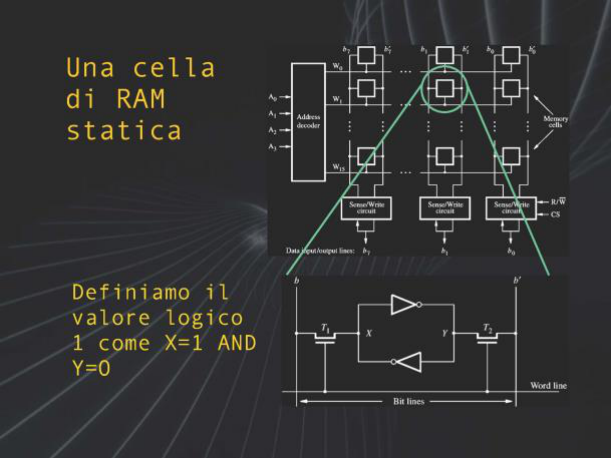
\includegraphics[width=0.80\textwidth,
                    trim=40 40 10 40, % L B R T
                    clip]
                    {images/Lez04_p03_fig_03.png}
  \caption{Static RAM}
  \label{fig:Lez04_p03_fig_03}
\end{figure}
\FloatBarrier
\noindent

Ritorniamo al nostra chip di prima in cui abbiamo detto che questo è un generico elemento di memoria e consideriamo che essa sia una cella di natura statica, quindi la generica cella è costituita da da due invertitori posti in contro in anello l'uno contro l'altro e acceduti da due pass transistor, cioè due transistori, che opportunamente aperti attraverso un segnale di tensione, quello che arriva sulla linea di parola, word line, vengono aperti e i dati che arrivano sulle linee di bit, ricordate avevamo due linee complementari, B e B', scrivono il dato contemporaneamente attraverso questi transistori.
Ovviamente deve valere che i segnali messi sulle linee B e B' siano complementari l'uno dell'altro.
Dal punto di vista pratico realizzativo questi invertitori sono realizzati in tecnologia CMOS, ma inizialmente vediamo che per esempio possiamo definire il valore logico 1 come la variabile x, lo stato interno uguale a 1, e dal punto di vista strettamente logico la variabile y uguale a 0.
Lo stato logico 0 di questa cella sarà quindi scambiando i valori di x e y.

\FloatBarrier
\begin{figure}[H]
  \centering
  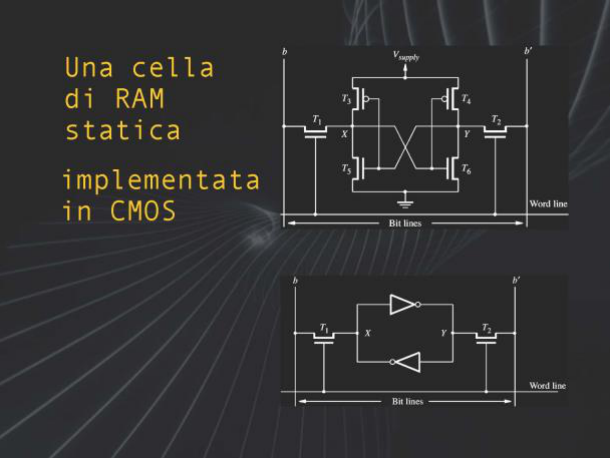
\includegraphics[width=0.80\textwidth,
                    trim=40 40 10 40, % L B R T
                    clip]
                    {images/Lez04_p03_fig_04.png}
  \caption{Riduzione numero pin}
  \label{fig:Lez04_p02_fig_04}
\end{figure}
\FloatBarrier
\noindent

Quindi la implementiamo in CMOS e per implementare CMOS i due invertitori non sono altro che i classici invertitori CMOS connesse le uscite con gli ingressi, e questo corrisponde esattamente alla rappresentazione dal punto di vista logico di questi due buffer invertitori, stati invertitori.

Vi invito a riflettere quali siano le principali problematiche delle SRAM.
Vi chiedo se possiamo usarle sempre.

\subsection{RAM dinamiche}

Prossimo argomento che è quello delle RAM dinamiche.

\FloatBarrier
\begin{figure}[H]
  \centering
  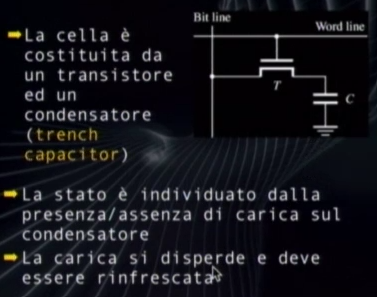
\includegraphics[width=0.70\textwidth,
                    trim=0 0 0 0, % L B R T
                    clip]
                    {images/Lez04_p03_fig_06a.png}
  \caption{Riduzione numero pin}
  \label{fig:Lez04_p03_fig_06a}
\end{figure}
\FloatBarrier
\noindent

La cella di una RAM dinamica è costituita da un transistore ed un solo condensatore, questo condensatore è chiamato trench capacitors.
Quindi in questo caso c'è una wordline, una bitline, un transistor, un pass-transistor che abilita un percorso a bassa impedenza verso un condensatore quando la wordline è selezionata oppure stabilisce un livello di alta impedenza e quindi isola la carica che è immagazzinata su questo condensatore.
Lo stato logico è individuato dalla presenza o assenza di carica sul condensatore.
Ovviamente presenza e assenza sono definite rispetto a una qualche soglia che discrimina un livello alto da un livello basso di tensione, quindi dalla presenza di una carica o dall'assenza di una carica.
Dal punto di vista la carica si disperde e quindi deve essere rinfrescata di tanto in tanto.
Questo è uno dei punti più critici delle DRAM perché mentre l'invertitore CMOS nella cella SRAM che avevamo visto prima, fintanto che l'alimentazione rimane, lo stato rimane tal quale non è modificato a prescindere dalla lettura, in questo caso vedremo che lo stato decade sia quando viene letto che a prescindere dalla lettura semplicemente perché il transistorio ha delle perdite, o  per la stessa realizzazione del condensatore che ha delle perdite.
Vi do una rappresentazione un po' schematica ma abbastanza importante di come è fatto questo transistore dal punto di vista fisico.

\FloatBarrier
\begin{figure}[H]
  \centering
  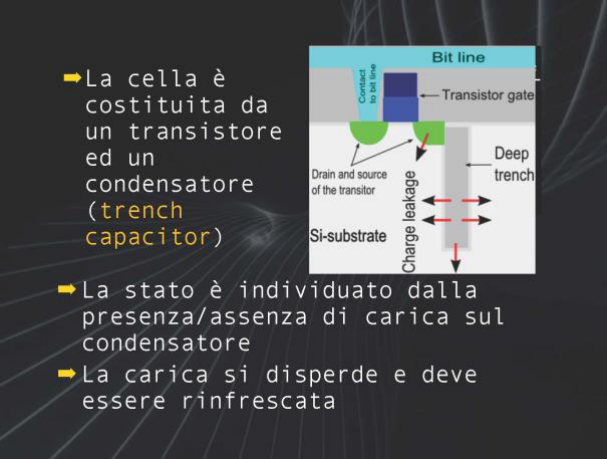
\includegraphics[width=0.70\textwidth,
                    trim=40 40 40 40, % L B R T
                    clip]
                    {images/Lez04_p04_fig_01.png}
  \caption{Riduzione numero pin}
  \label{fig:Lez04_p04_fig_ì1}
\end{figure}
\FloatBarrier
\noindent

Qua vediamo una bit line che è una pista metallizzata che contatta il drain cioè il collettore di un transistore MOS, qui c'è il gate o porta del transistore, questo è l'ossido di gate, qui c'è il source o sorgente del transistore che connette attraverso questa struttura che in inglese si chiama recess cioè scavata profondamente, è un deep trench, una profonda trincea, letteralmente significa profonda trincea in cui è stato scavato un buco nel silicio, nel substrato di silicio, è stato depositato un conduttore attorno al buco, è stato depositato uno strato di dielectrico, diciamo un ossido per esempio dell'ossio silicio anche se ormai non è più soltanto ossio silicio e sopra è stata applicata un'ulteriore metallizzazione per realizzare il secondo piatto del condensatore, questa struttura è connessa a massa attraverso l'elettrodo, diciamo attraverso la superficie esterna del condensatore ed è connesso al source del transistore attraverso l'elettrodo depositato sopra, quindi notate che ovviamente la struttura non è perfettamente in scala però rappresenta un po' il principio, per guadagnare in superficie e quindi in capacità del transistore è necessario realizzare un buco profondo per aumentare la superficie complessiva, questo è un processo che rende il processo leggermente diverso rispetto al normale processo CMOS e quindi le memorie DRAM vengono realizzate su linee generalmente non perfettamente standard rispetto a quelle dei comuni processori, cioè che realizzano CMOS, su questo torneremo più avanti quando parleremo di un particolare tipo di cache, le cosiddette embedded DRAM, in questo momento è importante per voi sapere che generalmente questa tecnologia non è pienamente compatibile con quella con cui si realizzano i microprocessori.

La cella è molto semplice, qui c'è una sola cella di porta mentre ne avevamo due nella SRAM, c'è un solo condensatore di memoria mentre ne avevamo quattro, due CMOS controreazionati nel caso della SRAM.

\FloatBarrier
\begin{figure}[H]
  \centering
  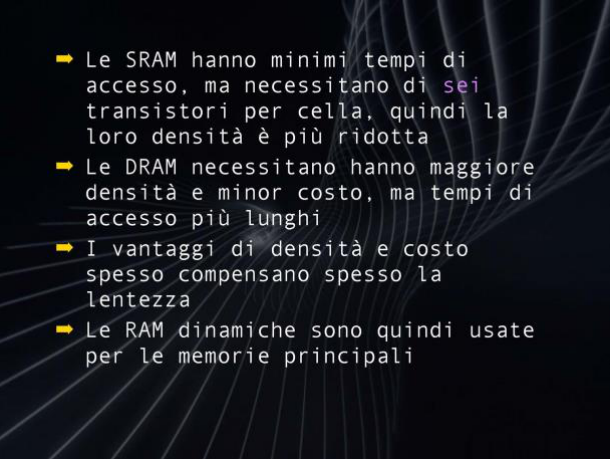
\includegraphics[width=0.70\textwidth,
                    trim=0 0 0 0, % L B R T
                    clip]
                    {images/Lez04_p04_fig_02.png}
  \caption{Confronto SRAM-DRAM}
  \label{fig:Lez04_p04_fig_02}
\end{figure}
\FloatBarrier
\noindent



Ripetiamo il concetto, 

le SRAM hanno minimi tempi di accesso perché il dato è già scritto ma necessitano di ben sei transistori per cella, quindi la densità è più ridotta di quanto non sia possibile ottenere con le DRAM che possono avere una maggiore densità e minor costo, perché il costo è legato sostanzialmente al numero dei passi e alla densità degli elementi che si trovano per unità di area ma hanno generalmente i tempi di accesso più lunghi perché è necessario leggere la scarica esponenziale del condensatore attraverso i circuiti di SENSE e al contrario delle SRAM che si comportano sostanzialmente come dei generatori di tensione, cioè l'uscita diretta degli stadi CMOS.

Analogamente la scrittura è fatta attraverso la carica di un condensatore che anche questa avviene con un andamento esponenziale, quindi sostanzialmente la natura intrinseca della scarica e della carica di un condensatore determina dei tempi di lettura e scrittura più lunghi.

Però in generale i vantaggi di densità e costo delle DRAM compensano quasi sempre, spesso almeno, la lentezza intrinseca del processo e quindi le RAM dinamiche sono utilizzate per le memorie principali delle architetture di elaborazione in quasi tutti i casi, salvo in quei casi tipo piccoli microcontrollori a basso consumo, dove si preferisce utilizzare ancora delle SRAM perché in condizioni diciamo normali, senza commutazione, non sono soggetti a significative perdite di potenza. Al contrario le DRAM devono essere rinfrescate e quindi intrinseicamente dissipano.
%25:01
Vediamo quindi il funzionamento dei chip di RAM dinamiche.
In lettura la carica della cella sulla riga selezionata è misurata dai circuiti di sense, cioè leggendo la capacità, 1 o 0 se la carica è al di sopra o al di sotto di una soglia.
La lettura stessa altra alla carica della cella e quindi impone il rinfresco della riga, quindi è necessario leggere la riga e prendere il valore e riscriverlo nuovamente attraverso la linea di bit, in questo caso una sola linea di bit.
In scrittura si accede alla riga e si pilotano le righe di bit, diciamo di tutta la parola.
Anche questa scrittura viene coi tempi caratteristici della carica di un condensatore, cioè comune esponenziale.
Occorre rinfrescare periodicamente anche se nulla viene letto, perché, come vi ho detto, vi è una intrinseca dissipazione attraverso il dielectrico del condensatore e attraverso, eventualmente anche se in piccola, quantità attraverso la porta del transistor che abilita il condensatore.
Vediamo quindi come è realizzata una drum, in questo caso 32 Mega per 8, questo chip.
In questo caso vediamo via un row address latch, un column address latch, cioè un latch che memorizza temporaneamente la parte di riga e la parte di colonne, gli indirizzi sono separati fra riga e colonne, si utilizzano due segnali che saranno fondamentali per chiunque pensa di guardare una memoria, i cosiddetti RAS e CAS, row address strobe e column address strobe ancora attivi bassi, vi è un decoder degli indirizzi di riga che seleziona la cella, analogamente un decoder di colonna, in questo caso avevamo un multiplexer, nell'altro caso in questo caso utilizziamo un decoder, ma vedete che non cambia molto nella questione, e ancora nuovamente i circuiti di sensor ride, la nostra cella costituita di 16.384 righe per 2.048 colonne, cioè 11 linee di bit per le colonne e 24 per le righe, quindi il progettista ha preferito utilizzare questo, scusate non 24, ma 14 linee di riga e 11 di colonna, in questo caso vedete in 14 bit per selezionare righe e 11 per selezionare la colonna.
Per risparmiare i pin è possibile multiplare le righe e le colonne sugli stessi i piedini, anche nelle drum, e questo è quello che tipicamente avviene, perché i piedini sono importanti, perché determinano il costo del circuito, i leccio di riga e colonna memorizzano i bit di indirizzo per tenere gli indirizzi più stabili, i segnali di memorizzazione degli indirizzi di riga e di colonna sono assediti bassi, notate che la multiplazione di indirizzi di riga e di colonna di fatto impone l'esistenza di almeno un leccio, in questo caso ne utilizziamo due, perché prima scriviamo l'indirizzo di riga, poi selezioniamo l'indirizzo di colonna, è chiaro che l'indirizzo di riga deve essere in qualche modo memorizzato.
Queste sono le cosiddette drum asincrone, hanno un ritardo di accesso legato ai tempi di scrittura delle righe e di colonne, un controllore esterno legge e periodicamente rinfresca tutte le memorie, sono state le prime drum a essere utilizzate.
Nell'esempio precedente tutte le 16.384 celle su una riga vengono accedute contemporaneamente e rinfrescate periodicamente perché il dato venga mantenuto.
Notate che però solo 8 bit di dati vengono trasferiti per ogni ciclo di indirizzamento e di riga, quindi ogni volta bisogna applicare un RAS e un CAS per prendere una semplice parola di 8 bit di dato.
Notate che quindi sono necessarie due operazioni di scrittura sul basso indirizzo per accedere a un dato in lettura o scrivere il dato in fase di scrittura.
Vi accorgete che questo ha chiaramente dei costi in termini di tempo e vi do quindi il solito spunto per la riflessione e vi invito a pensare come si potrebbe incrementare la velocità rispetto al funzionamento asincrono.
Prendete ora un attimo il vostro tempo prima di proseguire nella lezione e riflettete a questa domanda.
Riflettete un attimino che poi la risposta ve la do, però non proseguite nella lezione senza esservi un attimo sforzati.
Passiamo quindi ad affrontare l'argomento delle RAM SYNCHRON o Synchronous Dynamic RAMs RAM in inglese.
Nei primi anni 90 la tecnologia delle DRAM migliorò con l'introduzione di un segnale di clock all'ingresso delle DRAM.
Fu aggiunta ulteriore circuiteria per la sincronizzazione e questi circuiti integrati così sincronizzati da un clock sono chiamati Synchronous DRAM o DRAM.
Vediamo come è costituita questa DRAM diciamo nella configurazione semplice.
Ancora abbiamo il raw address latch perché le righe e le colonne sono multiplexate e l'abilitazione è sempre determinata da RAS e CAS.
Però in aggiunta al raw address latch, cioè l'atch dell'indirizzo di riga, si mette un contatore di rinfresco che va a scandire quindi gli indirizzi.
Quindi questo è un contatore aggiuntivo.
C'è un ulteriore contatore di colonne e poi a valle di questi vi sono dei decoder.
Qui c'è la cella di array e quindi qui ancora i vari circuiti di read write, sense e dei latch.
La cosa interessante è che in uscita non vi è l'uscita direttamente attraverso un decoder o un multiplexer come abbiamo visto precedentemente, ma vi sono dei registri, dei registri synchroni rispetto al clock.
Qui è un data input register, cioè un registro in fase di ingresso e un registro in fase di uscita.
Una sequenza di circuterie aggiuntive che producono i sincronismi per tutto questo circuito clock, RAS e CAS negati, read write e chip select.
Quindi il sistema aumenta in termini di variabili in ingresso perché c'è anche il clock e soprattutto aumenta perché vi sono due registri dei dati e due contatori per definire gli indirizzi che non vengono più mandati semplicemente ma vengono anche aggiornati internamente.
In questo caso i circuiti di sense hanno una funzione di latching del dato e ulteriori vantaggi da immagazzinamento interno e disponibilità di clock e di sincronizzazione permettono di aumentare il flusso dei dati, la velocità del flusso dei dati.
Il contatore di riga interno consente il rinfresco delle celle di memoria indipendentemente da un controllore esterno.
Come avevo detto nelle drum asincrone era necessario produrre da un controllore esterno la sequenza con RAS e CAS per rinfrescare tutta la celle.
In questo caso deve solo arrivare un comando di rinfresco, il refresh counter fa la scansione degli indirizzi di riga e quindi vengono rischiti qua, si fa la scansione della celle e analogamente il contatore di indirizzi di colonna fa il rinfresco.
E quindi è anche possibile fare il rinfresco senza dover mandare in continuazione dall'esterno i segnali di riga, colon, RAS e CAS.
Notate che questo oltre ad avere una semplificazione per il controllore della memoria esterna, riduce anche il consumo di potenza perché non è più necessario scrivere ripetutamente gli indirizzi di riga e di colonna e asserire RAS e CAS attraverso magari delle piste lunghe diverse centimetri, quindi dotate di una capacità e per ogni capacità c'è un mezzo CV quadro di energia dissipata per ogni commutazione.
In questo caso viene tutto realizzato internamente e quindi può procedere più rapidamente oppure semplicemente dissipare meno.
In generale sono vere entrambe le cose, cioè si dissipa meno e si può realizzare il rinfresco in maniera più rapida.
E' importante che l'esistenza dei contatori di colonna permettono di scandire la riga e non si possa dover riasserire nuovamente il segnale di ROW ad DRE STROBE per indirizzi contigui sulla stessa riga.
Questo permette il trasferimento di più parole aventi della stessa riga di indirizzo ma colonne consecutive.
Questo fa sì, come ho detto, che non è necessario riasserire ripetutamente RAS.
Vediamo quindi che le SRAM, come ho detto, includono registi di dati oltre che l'Hatch per gli indirizzi.
Le nuove operazioni di accesso possono essere iniziate quando le precedenti sono ancora in transito grazie ai registi di ingresso e di uscita dei dati.
E le configurazioni dei circuiti di controllo delle SRAM, la configurazione richiede una però configurazione all'accensione, cioè la SRAM deve essere educata sul da farsi.
Il controllore della memoria inizializza semplicemente la memoria ma non deve più nuovamente rinfrescarla come avviene nelle DRAMs asincrone.
Specifica inoltre il controllore, la lunghezza per il trasferimento a blocchi e i ritardi necessari per l'asincronizzazione.
Questo consente di ottenere trasferimenti a blocchi efficienti.
Le DRAMs asincrone incorrono infatti i ritardi dovuti all'assersione di RAS e CAS per ogni indirizzo di colonna.
In realtà, mentre nelle SRAM si riducono i ritardi asserendo colon address strobe solo per l'indirizzo iniziale di colonna e poi il contatore interno dei registi di colonna aggiorna gli indirizi e decodifica elementi sulla stessa riga di indirizzo ma con colonne consecutive.
Il trasferimento a blocchi, abbiamo detto, è efficiente perché la circuteria delle SRAM incrementa il contatore di colonna e trasferisce automaticamente dati consecutivi.
La lunghezza del BARST determina la lunghezza del trasferimento.
BARST è un evento improvviso e veloce.
Consideriamo ora, come esempio semplificato, un BARST di lunghezza 4, ritardo nel RAS di 3 cicli e di CAS nei 2 cicli.
Questo è un esempio molto semplificativo ma ci permette di rappresentarlo graficamente sullo schermo.
Nella realtà i ritardi sono sensibilmente più lunghi ma è utile dal punto di vista didattico.
Guardiamo quindi l'oscillogramma della nostra memoria in cui abbiamo un clock, i segnali di read-write, RAS e CAS negati, le linee di indirizzo e le linee di dati.
Questa terminologia ci dice che qui avviene il dato, qui vengono messi gli indirizzi di riga, qui vengono messi gli indirizzi di colonna rispetto al clock, qui vengono prodotti i dati, quindi il resto dei dati e in alta impedenza non interessa, il segnale read-write alto, alto sta per read, il segnale RAS e CAS sono assediti bassi, notate che RAS è assedito prima perché prima si mandano gli indirizzi di riga, vedete il ritardo tra RAS e CAS è di tre cicli perché il tempo che RAS è assedito non si può assedire CAS prima che partano almeno tre cicli.
Dopo che è assedito CAS con due cicli di latenza, compaiono i dati, quindi vedete che dopo l'assersione di CAS, le linee di dati sono assedite.
Dopo due cicli sono disponibili i dati, questo è un esempio molto semplificativo, altrimenti avremmo avuto questo grafico molto più largo e meno visibile, infine abbiamo deciso che il nostro BARS è costituito di quattro dati che vengono tirati fuori sincroni sul fronte positivo del clock e quindi raccolti.
Notate che se avessimo dovuto riassedire RAS e CAS per ognuno di questi dati, chiaramente i tempi sarebbero stati sensibilmente più lunghi.
Vi invito a fare il calcolo del vantaggio temporale avendo mantenuto le stesse tempistiche di RAS e CAS, quindi tre cicli per RAS e due di CAS, quanti cicli complessivi servirebbero nel caso in cui la memoria sia completamente asincrona invece che sincrona come la presente.
Con questo vi do uno spunto per la riflessione e vi chiedo come si potrebbe ulteriormente incrementare la velocità rispetto al funzionamento sincrono sul fronte del clock.
Con questo però questa curiosità ve la toglierò nella prossima lezione e quindi vi invito a riguardare con attenzione la lezione e a partecipare a seguire la prossima lezione che vi darà questa ed altre risposte.